\footnotesize
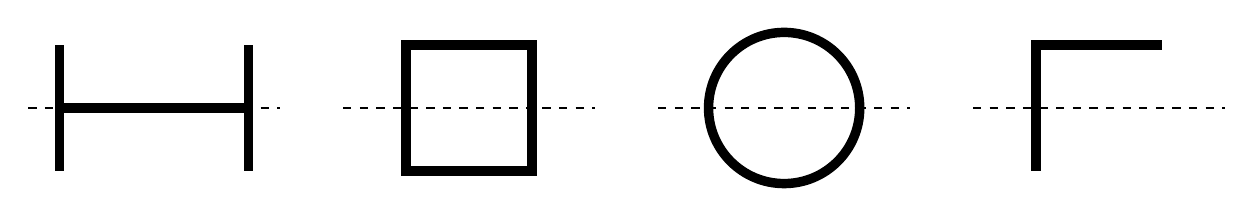
\begin{tikzpicture}[scale=.8]
\begin{scope}
\draw[line width=1.2mm](-1.5,-1)--++(0,2)(1.5,-1)--++(0,2)(-1.5,0)--++(3,0);
\draw[dashed](-2,0)--++(4,0);
\end{scope}
\begin{scope}[xshift=5cm]
\draw[line width=1.2mm](-1,-1)rectangle(1,1);
\draw[dashed](-2,0)--++(4,0);
\end{scope}
\begin{scope}[xshift=10cm]
\draw[line width=1.2mm](0,0)circle(1.2cm);
\draw[dashed](-2,0)--++(4,0);
\end{scope}
\begin{scope}[xshift=15cm]
\draw[line width=1.2mm](-1,-1)|-(1,1);
\draw[dashed](-2,0)--++(4,0);
\end{scope}
\end{tikzpicture}